\begin{figure}[ht]
\centering
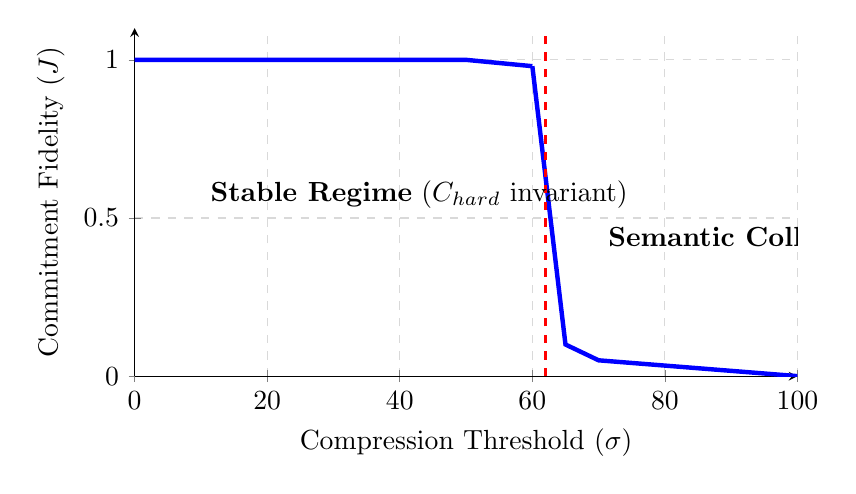
\begin{tikzpicture}
\begin{axis}[
    width=10cm, height=6cm,
    xlabel={Compression Threshold ($\sigma$)},
    ylabel={Commitment Fidelity ($J$)},
    xmin=0, xmax=100,
    ymin=0, ymax=1.1,
    xtick={0,20,40,60,80,100},
    ytick={0,0.5,1.0},
    axis lines=left,
    grid=major,
    grid style={dashed, gray!30}
]

% The Stability Plateau
\addplot[color=blue, ultra thick] coordinates {
    (0,1) (10,1) (20,1) (30,1) (40,1) (50,1) (60,0.98)
};

% The Collapse (Phase Transition)
\addplot[color=blue, ultra thick] coordinates {
    (60,0.98) (65,0.1) (70,0.05) (100,0)
};

% Annotations
\draw[red, dashed, thick] (axis cs:62, 0) -- (axis cs:62, 1.1) node[above] {$\sigma_c$ (Collapse Threshold)};
\node[anchor=south west] at (axis cs:10, 0.5) {\textbf{Stable Regime} ($C_{hard}$ invariant)};
\node[anchor=north west] at (axis cs:70, 0.5) {\textbf{Semantic Collapse}};

\end{axis}
\end{tikzpicture}
\caption{Commitment fidelity as a function of compression threshold. The system exhibits a phase transition at $\sigma_c$, where commitment conservation abruptly fails. Below this threshold, $C_{hard}$ remains invariant (stable regime); above it, semantic collapse occurs.}
\label{fig:commitment-stability}
\end{figure}
